\begin{center}
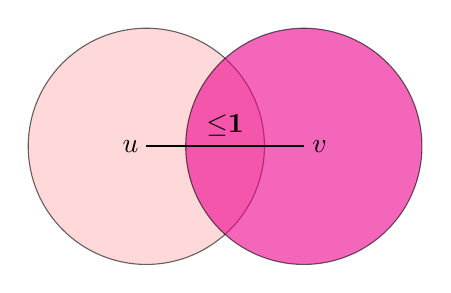
\begin{tikzpicture}

    % Draw the first circle (pink)
    \draw[fill=pink, opacity=0.6] (0,0) circle (1.5cm); 
    \node at (-0.2, 0) {\textbf{$u$}}; % Label the center as u
    
    % Draw the second circle (magenta) touching the first
    \draw[fill=magenta, opacity=0.6] (2,0) circle (1.5cm);
    \node at (2.2, 0) {\textbf{$v$}}; % Label the center as v
    
    % Draw the line between the centers and label it
    \draw[thick] (0,0) -- (2,0) node[midway, above] {\textbf{$\le$1}};
    
\end{tikzpicture}
\end{center}